\documentclass[11pt]{article}
\usepackage{colacl}
\usepackage{graphicx}
\usepackage[T1]{fontenc}
\usepackage[utf8]{inputenc}
\graphicspath{{img/}}
\DeclareUnicodeCharacter{F8FF}{$\diamond$}
\sloppy

\title{COMP30027 Assignment 2: Report}
\author
{Anonymous}



\begin{document}
\maketitle

\section{Introduction}
% Introduction: a short description of the problem and data set

The dataset provided contains two lists of {T}witter posts (tweets) made on the platform prior to 2017 \cite{dataset}.
Each tweet is an instance in the dataset.
The two files enclosed in the dataset are a \texttt{Train.csv} for training and a \texttt{Test.csv} for testing. 
For each Tweet, included is the text and its ID. 
Included in the training file is also a column containing the sentiments of the tweets. 
Tweets can either have a "positive", "neutral" or "negative" sentiment.
The goal was to develop and train an accurate classifer model using the dataset and apply it to the testing set.

\section{Methodology}
% Method: Introduce the used feature(s), and the rationale behind including them. Explain the classifiers
% and evaluation method(s) and metric(s) you have used (and why you have used them). This should be
% at a conceptual level; a detailed description of the code is not appropriate for the report. The description
% should be similar to what you would see in a machine learning conference paper.

\subsection{Raw Data Analysis}
First, the dataset was looked at based on the raw data as it came.
The training set contains $21802$ labelled instances and the testing set contains $6099$ instances. 
The raw tweets are strings of lowercase text and contain misspelled words, non-alphanumeric characters, Twitter-specific features (mentions and hashtags), and foreign language.

The distribution of the sentiment labels across the training set was also considered, 
displaying a clear majority of neutral tweets \ref{fig:sent-dist}.

\begin{figure}[!h]
	\centering
	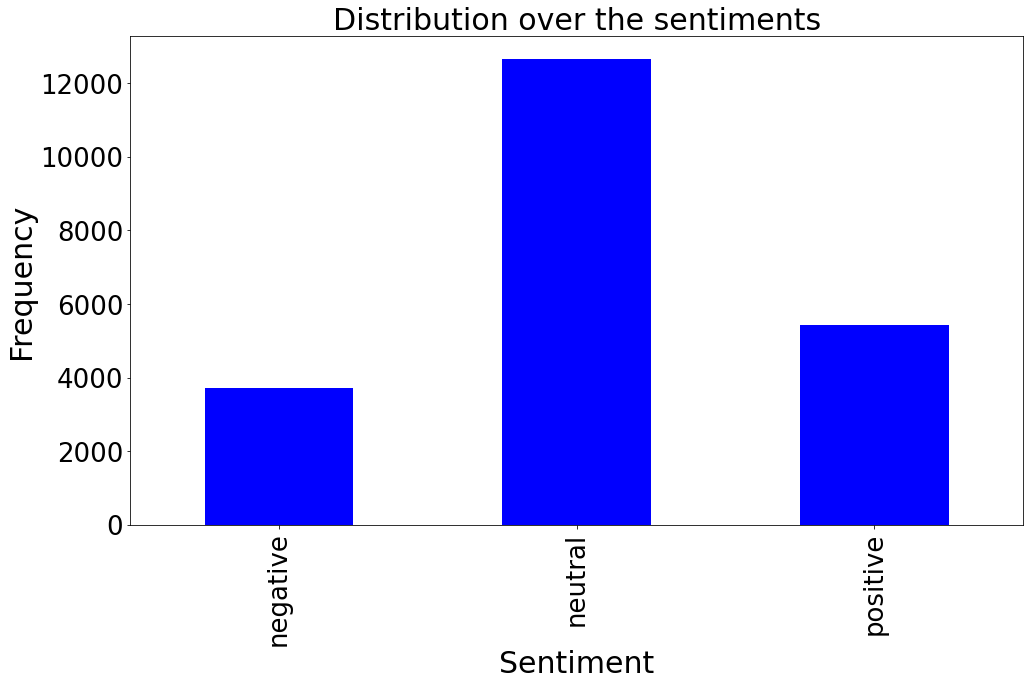
\includegraphics[width = 0.45\textwidth]{sentiment-distribution.png}
	\caption{Distribution of the sentiments}
	\label{fig:sent-dist}
\end{figure} 

\subsection{Preprocessing}

\subsubsection{Cleaning}
Some features required the text instances be cleaned before extraction.
Cleaning involves pruning the tweet of certain characters and features to varying degrees.
Usually, this means isolating only the alphabetic characters in the text, and performing simple casefolding.
Since all instances in the dataset are lowercase, only removal of unwanted characters was necessary.
A type of cleaning considered was the removal of repeated consecutive characters.
An example where this may have been useful is when encountering words such as \texttt{hey}, which can also appear as \texttt{heyyy}.
One issue with this method of avoiding suffixing is that it can change the meanings of certain words. For example, \texttt{good} becomes \texttt{god}.
Extreme suffixing can also be circumvented through stemming or lemmatization, which are discussed in Sections~\ref{sec:stems} and \ref{sec:lemmas}.

% However, consecutive repeated character pruning was arguably just a primitive, 
% but language-agnostic implementation of stemming or lemmatization, which are discussed in Section~\ref{subsection:tokens}.
% Determining the best 

\subsubsection{Stopwords}

Initially, the dataset was analyzed to see how different words are distributed throughout it.
This yielded a word cloud over both the training and testing sets, with the most common words being considered for the stopword list (Figure~\ref{fig:wc-all}).

\begin{figure}[!h]
	\centering
	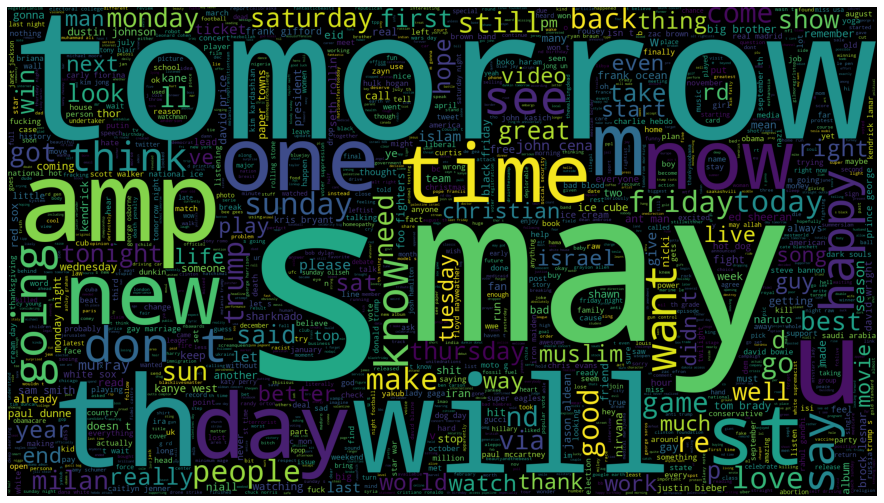
\includegraphics[width = 0.45\textwidth]{wc-all-clean-default.png}
	\caption{Word cloud over all tweets}
	\label{fig:wc-all}
\end{figure} 

The construction of the list was contextual, as some words that appear frequently may still be useful for sentiment analysis.
To get a better picture of these common, but useful words, three more word clouds were constructed over the word lists per sentiment (Figures~\ref{fig:wc-pos}, \ref{fig:wc-neu}, and \ref{fig:wc-neg}).

\begin{figure}[!h]
	\centering
	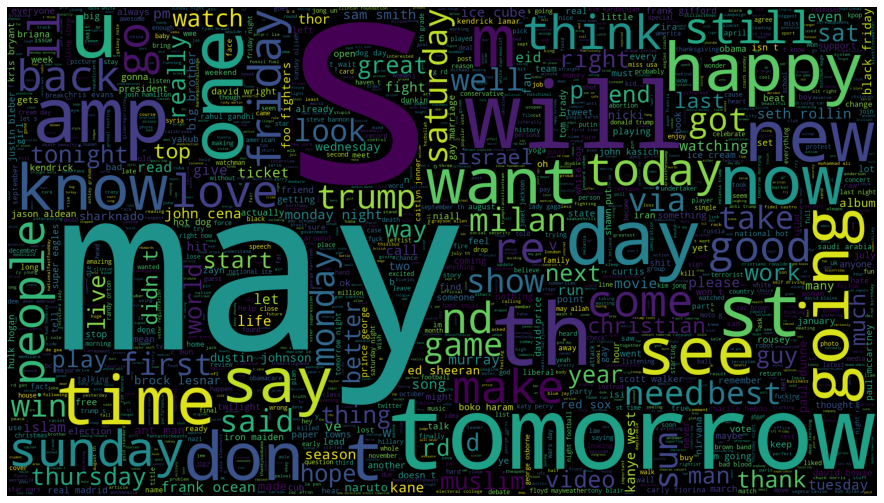
\includegraphics[width = 0.45\textwidth]{wc-positive-clean-default.png}
	\caption{Word cloud over positive training tweets}
	\label{fig:wc-pos}
\end{figure} 

\begin{figure}[!h]
	\centering
	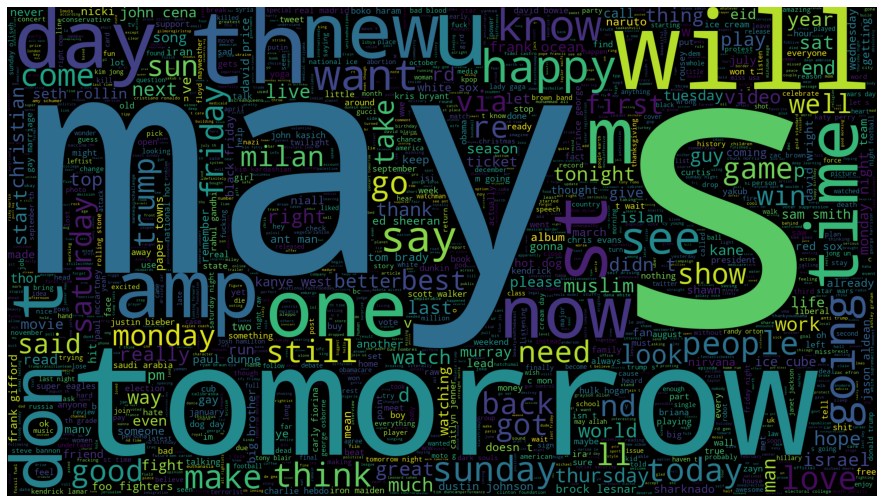
\includegraphics[width = 0.45\textwidth]{wc-neutral-clean-default.png}
	\caption{Word cloud over neutral training tweets}
	\label{fig:wc-neu}
\end{figure} 

\begin{figure}[!h]
	\centering
	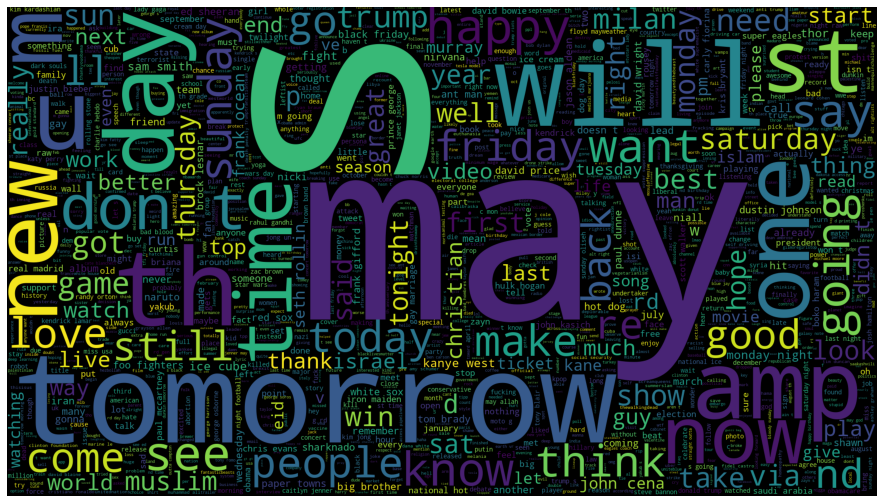
\includegraphics[width = 0.45\textwidth]{wc-negative-clean-default.png}
	\caption{Word cloud over negative training tweets}
	\label{fig:wc-neg}
\end{figure} 

However this method did not consider stopwords in other languages (since english tweets are an overwhelming majority in the dataset).
Since manual stopword list construction was not as exhaustive as the data required,
the {P}ython \texttt{NLTK} module's stopword corpus is used where necessary \cite{nltk}.

\subsection{Vectorization}

Classifiers in the \texttt{SciKit-learn} {P}ython library require that all data be vectorized to a real-valued space.
The following vectorizers were used.

\subsubsection{Count}

Vectorising the tweet into term counts can highlight terms which appear more often in tweets for certain sentiments.
This is implemented using \texttt{SciKit-learn}'s \texttt{CountVectorizer} \cite{skl}.

\subsubsection{TF-IDF}

This measure of relative word frequency provides more insight, 
as it measures words that appeach more often in one tweet relative to their overall frequency.
This is implemented using \texttt{SciKit-learn}'s \texttt{TfidfVectorizer} \cite{skl}.

\subsubsection{Metrics}

The final type of vectorization that will occur is in the form of metrics. 
Certain metrics such as world length may be distributed differently based on the sentiment of the tweet.
This is implemented by creating a list of mappings to metrics, then vectorizing with \texttt{SciKit-learn}'s \texttt{DictVectorizer} \cite{skl}.

\subsubsection{Why not hashing?}

The \texttt{SciKit-learn} library suggests another text feature extractor in the form of hashing.
This is not used here as the distinct advantage this vectorizer has over others is saving on space and time \cite{skl}.
While the dataset contains more than 20000 tweets, using the other vectorizers did not present such issues in practice.

\subsection{Features}\label{subsection:tokens}

While the data is given as a raw text format, there are multiple features which can be extracted for the purpose of sentiment analysis.

\subsubsection{N-grams}

This includes extraction of individual words or characters (1-grams of each) and word pairings (2-grams).
If $N > 1$, important orderings/configurations of words can be identified, but at the cost of exponentially increasing the possible number of features.
With a vocabulary of $w$ unique words, there can be as many as $w^N$ distinct N-grams.
Therefore, the N-grams used for model construction are:
\begin{itemize}
	\item 1-grams of words,
	\item 1-grams of characters,
	\item 2-grams of words.
\end{itemize}

This method will requires that tweets are cleaned, but may not need stopword removal.

\subsubsection{Stems}\label{sec:stems}
Can find the roots for english words by removing stems. It can also be used as a cleaning step.
However, this may be less effective with words that aren't in english (as they may use different suffixes),
or words which are misspelled.

\subsubsection{Lemmas}\label{sec:lemmas}
This method finds the true roots of words. This suffers from the same drawback as stemming, relying the text being in english.

\subsubsection{Word Lengths}

A tokenization where the tokens generated are the lengths of the words in the tweet.

\subsubsection{Character Frequencies}

\subsubsection{Links}

\subsubsection{Hashtags}

\subsubsection{Mentions}

\subsubsection{Emoticons}

\subsubsection{Simple Metrics}

\subsubsection{Phonetic Frequencies}

\subsubsection{Poetic Phonetics}

\subsection{Model Selection}

\subsubsection{Feature Selection}

\subsubsection{Classifiers}

\subsubsection{Evaluation Metrics}

\section{Results}
% Results: Present the results, in terms of evaluation metric(s) and, ideally, illustrative examples and diagrams.

\section{Analysis}
% Discussion / Critical Analysis: Contextualise the systems' behaviour, based on the understanding of the
% subject materials (This is the most important part of the task in this assignment).

% Contextualise implies that we are more interested in seeing evidence of you have thought about the task
% and determining reasons for the relative performance of different methods, rather than the raw scores of
% the different methods you selected. This is not to say that you should ignore the relative performance of
% different runs over the data, but rather that you should think beyond simple numbers to the reasons that
% underlie them.

\section{Conclusions}
% Conclusion: Demonstrate your identified knowledge about the problem.

\bibliographystyle{acl}
\bibliography{citations}

\end{document}
